\section*{2. Prediction Space Ablation (EC2)}

\subsection*{Problem \& Approach}
\textbf{Main HW3 uses x-prediction}: the network predicts $\hat{x}$ with weighted loss $\|(\hat{x}-x)/(1-t)\|^2$, then samples via Euler with $v = (\hat{x}-z_t)/(1-t)$. EC2 ablates this choice against $\varepsilon$-prediction and v-prediction on the same unconditioned EmojiViT. Following Li \& He (2025), we ask whether $\varepsilon$-prediction fails most without time conditioning---the same no-time setup main HW3 relies on.

\subsection*{Results}

\begin{table}[h]
\centering
\begin{tabular}{l c c l}
\toprule
\textbf{Parameterization} & \textbf{Final Train Loss} & \textbf{Final Val Loss} & \textbf{vs.\ Main HW3} \\
\midrule
\textbf{x-pred (main HW3)} & 0.1753 & 0.1910 & baseline method \\
$\varepsilon$-prediction & 0.0374 & 0.0294 & different loss scale \\
v-prediction & 0.1968 & 0.2066 & worse val than main \\
\bottomrule
\end{tabular}
\caption{EC2 at 300 epochs. Main HW3 at 500 epochs: train $= 0.1531$, val $= 0.1857$. x-pred EC re-train matches main HW3 at epoch 300 (val $= 0.1908$).}
\label{tab:ec2_loss}
\end{table}

\begin{figure}[h]
    \centering
    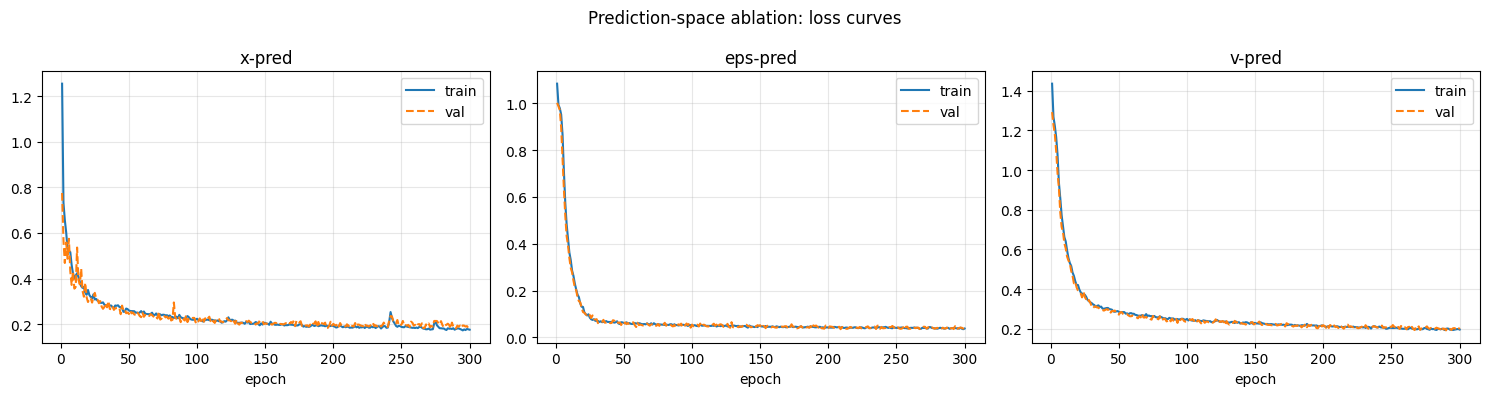
\includegraphics[width=0.95\textwidth]{figures/ec2_loss_curves.png}
    \caption{Per-method loss curves. x-pred (left) follows the same trajectory as main HW3 training.}
    \label{fig:ec2_loss}
\end{figure}

\begin{figure}[h]
    \centering
    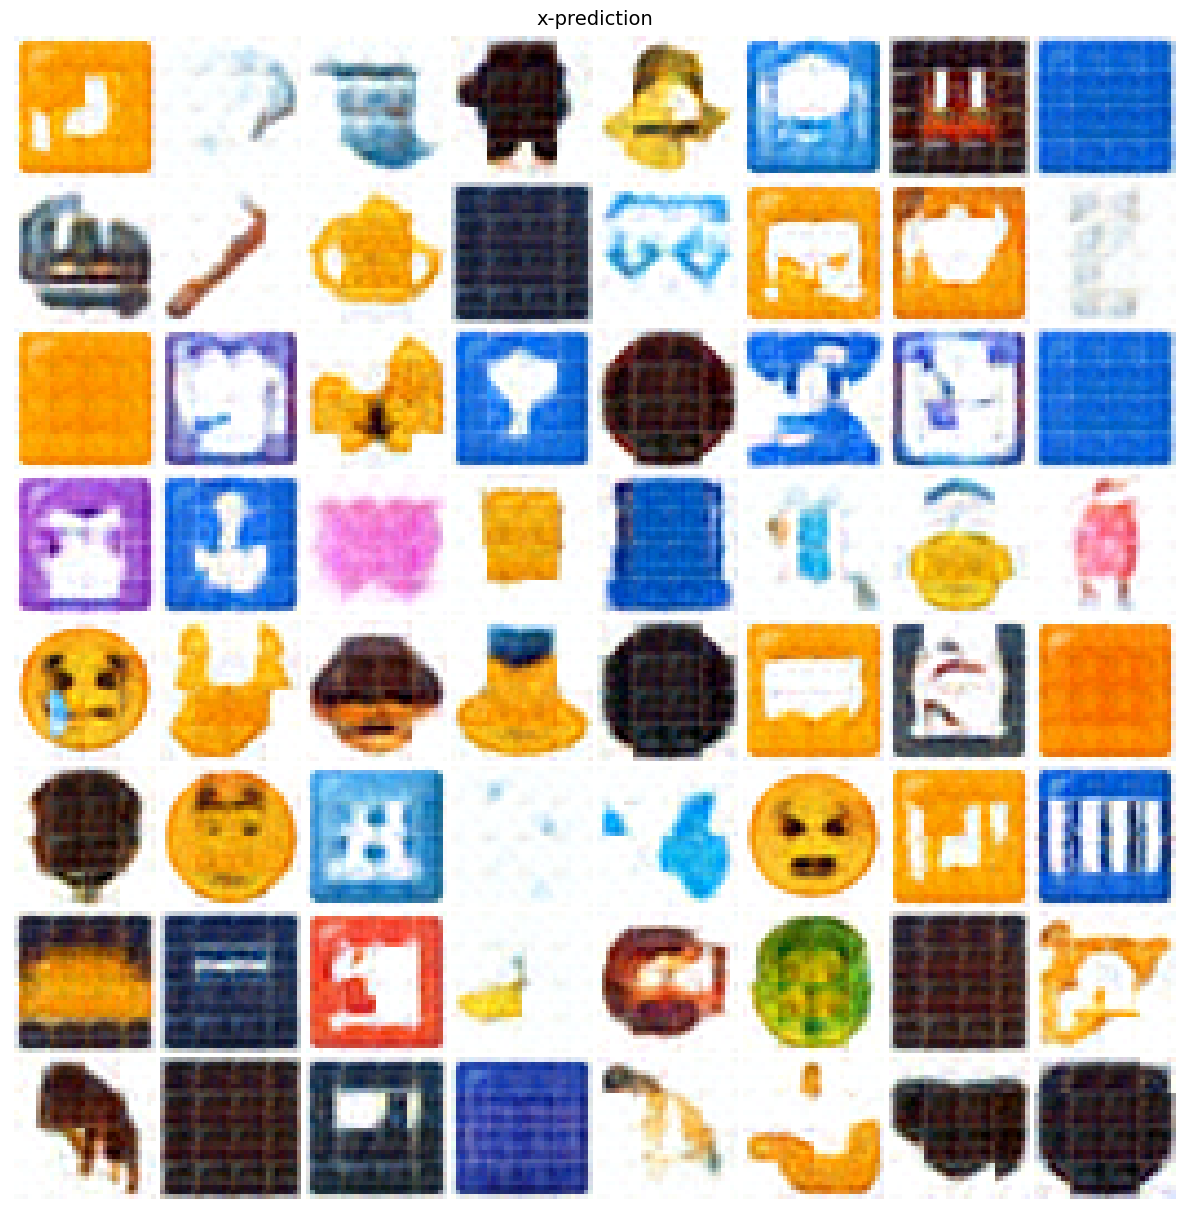
\includegraphics[width=0.32\textwidth]{figures/ec2_samples_x.png}
    \hfill
    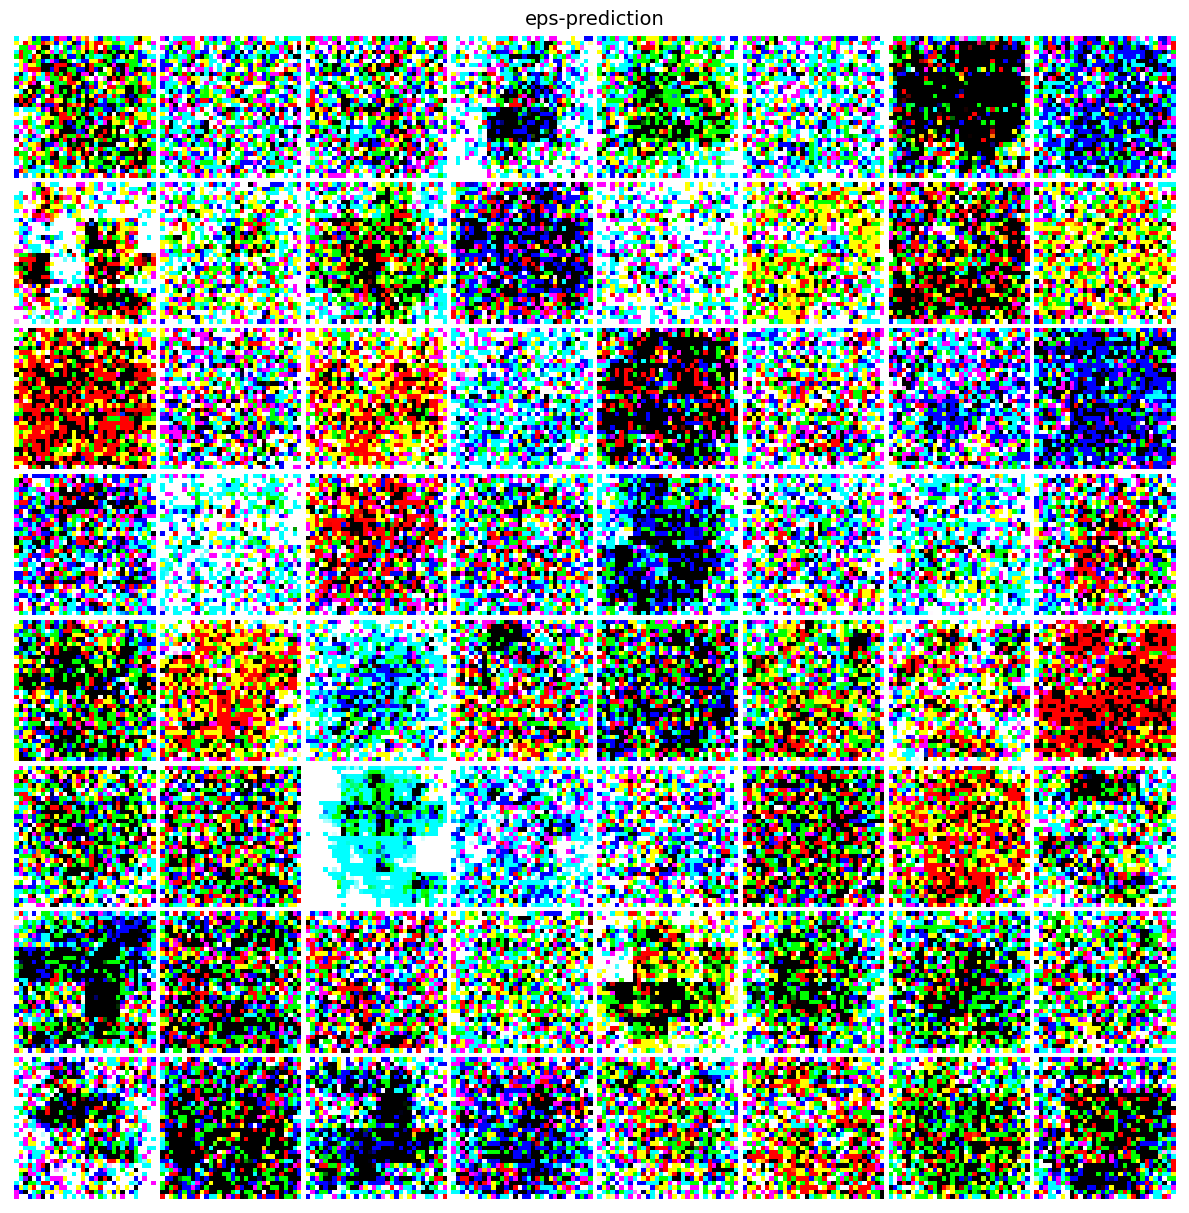
\includegraphics[width=0.32\textwidth]{figures/ec2_samples_eps.png}
    \hfill
    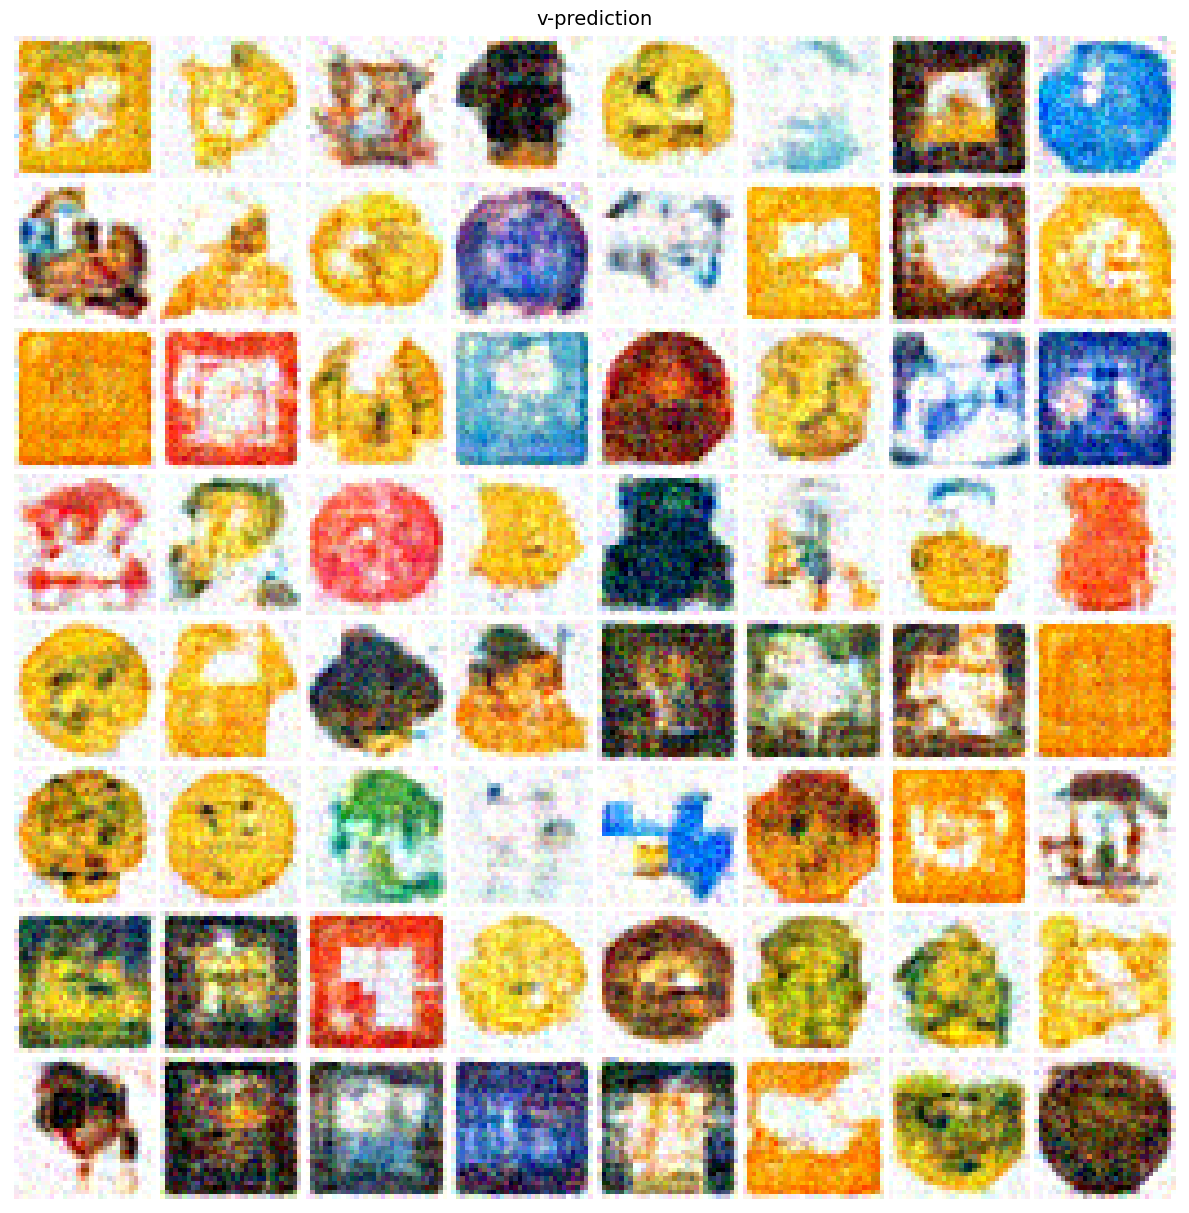
\includegraphics[width=0.32\textwidth]{figures/ec2_samples_v.png}
    \caption{x-pred (main HW3 method), $\varepsilon$-pred, v-pred samples. Only x-pred matches main HW3 quality (Figure~\ref{fig:main_samples}).}
    \label{fig:ec2_samples}
\end{figure}

\begin{figure}[h]
    \centering
    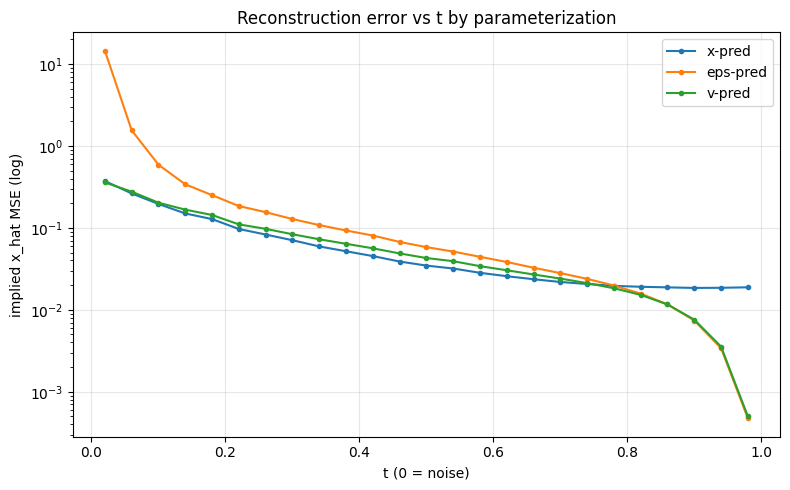
\includegraphics[width=0.75\textwidth]{figures/ec2_recon_vs_t.png}
    \caption{Implied $\hat{x}$ error vs.\ $t$. Main HW3's x-pred is stable; $\varepsilon$-pred blows up at small $t$.}
    \label{fig:ec2_recon}
\end{figure}

\subsection*{Discussion}
\textbf{x-prediction---main HW3's choice---is validated.} It produces samples comparable to the submitted main assignment and stable reconstruction across all $t$. $\varepsilon$-prediction fails despite low training loss: recovering $\hat{x} = (z_t - (1-t)\hat{\varepsilon})/t$ amplifies error by $1/t$ where the unconditioned network (same as main HW3) is weakest. This reproduces Li \& He (2025): without time conditioning, $\varepsilon$-prediction is the least robust. v-prediction is well-conditioned but slightly worse val loss than x-pred here; main HW3's x-pred parameterization is the right default for this setup.
